\section{迭代三工作项开展流程}
\begin{frame}
    \frametitle{优化SD服务缓存池策略}
    \begin{itemize}
        \item 在之前的单元测试和集成测试工作中,我们小组发现SD绘图的最大开销来源于从硬盘加载用户模型这一过程。因此在迭代三中,我们小组的SD服务维护人员重新设计了模型加载缓存池算法,采用LRU机制,在服务器缓存中维护若干之前用户的模型加载数据结构,并且在缓存池满且缓存未命中时,再从硬盘中将新模型加载到缓存,同时换出LRU队列中最近被加载频度最低的模型数据结构,从而有效提高了对于用户绘图请求的响应速度。在此基础上,我们小组的SD服务维护人员在经过反复的系统测试和实验后,最终将缓存池大小进行了合理设置,从而使得其既能够保证缓存池中的模型可以满足大部分的用户请求场景,同时也不会因为缓存池过大而导致内存占用过高,影响SD服务的运行性能。
    \end{itemize}
\end{frame}

\begin{frame}
    \frametitle{优化SD服务缓存池策略}
    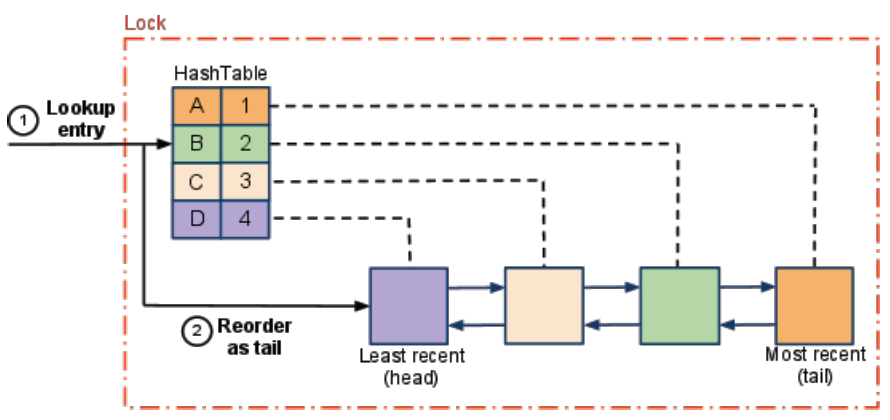
\includegraphics[width=\textwidth]{contents/figure/LRU.png}
\end{frame}

\begin{frame}
    \frametitle{Redis中间件缓存机制实现}
    \begin{itemize}
        \item 在迭代3中,我们小组在Tornado服务和MySQL服务之间,架设了Redis中间件,采用旁路缓存策略,在数据库事务到来时,首先在Redis中查询缓存,缓存未命中时再访问数据库,然后将数据库中的数据读出并且写入Redis缓存,从而有效减少了对于MySQL数据库的访问次数,提高了系统的运行性能。
        \item 同时,为了保证MySQL和Redis的数据一致性,我们小组在迭代3会议中经过讨论和架构设计,最终决定采用缓存延迟双删的策略,即在数据库事务执行前先删除缓存,然后在事务执行完毕后,延迟一段时间后再次删除Redis缓存。这样在一般的并发情境下,基本上在数据库服务中不会出现脏数据。
    \end{itemize}
\end{frame}

\begin{frame}
    \frametitle{生成图片合法性保证与检测}
    \begin{itemize}
        \item 在迭代2汇报与甲方的沟通中,甲方提出了一个对于生成图片合法性进行检验的项目需求。因此,我们小组的开发人员经过会议讨论,最终对于这一合法性检验需求,提出了采用Trie进行非法prompt字段匹配校验,从而过滤非法生成字符,并且在用户prompt中,引入prompt prefix装饰器机制,对于C端调用的prompt接口方法进行封装,从而控制OpenCLIP编码器产生的文本向量,在每个step的收敛过程中都能够保证生成的文本向量在prompt prefix的约束下进行的整套合法性检验解决方案,在最终的系统测试中,该方案能够有效保证生成图片的合法性,并且极大地提升了用户裸文本(raw text)输入情况下的生成图片质量。
    \end{itemize}
\end{frame}

\begin{frame}
    \frametitle{前端交互逻辑优化}
    迭代3开发工作中,我们小组负责前端开发的同学针对之前迭代2中前端交互逻辑的不足,对于前端的交互逻辑进行了优化,主要包括以下几个方面:
    \begin{itemize}
        \item 搜索界面中,支持了通过单击回车键进行搜索的交互逻辑。
        \item AI画图界面中,对于prompt文本进行了更加详细的描述,加入了提示性文本引导用户操作,避免用户使用时因为功能和参数过于复杂导致的困扰
        \item 修复了登录界面中,登录栏与注册栏在浏览器页面缩放下的错位问题。
        \item 修复了若干界面显示样式问题,使得整个系统的前端交互逻辑更加合理。
    \end{itemize}
\end{frame}

\begin{frame}
    \frametitle{单元测试}
    对于软件系统的单元测试,我们小组分别采用了使用Apifox工具和Python requests库请求的方式,请求每个实现接口对应的url,并且分别验证接口返回数据格式的正确性、接口根据实际业务请求内容做出响应的正确性和接口在高并发情景下的执行正确性。
    首先,Apifox接口测试流程大致如下。在每个接口定义中,填入参数并且发送,比如这里以/user/register接口为例:
    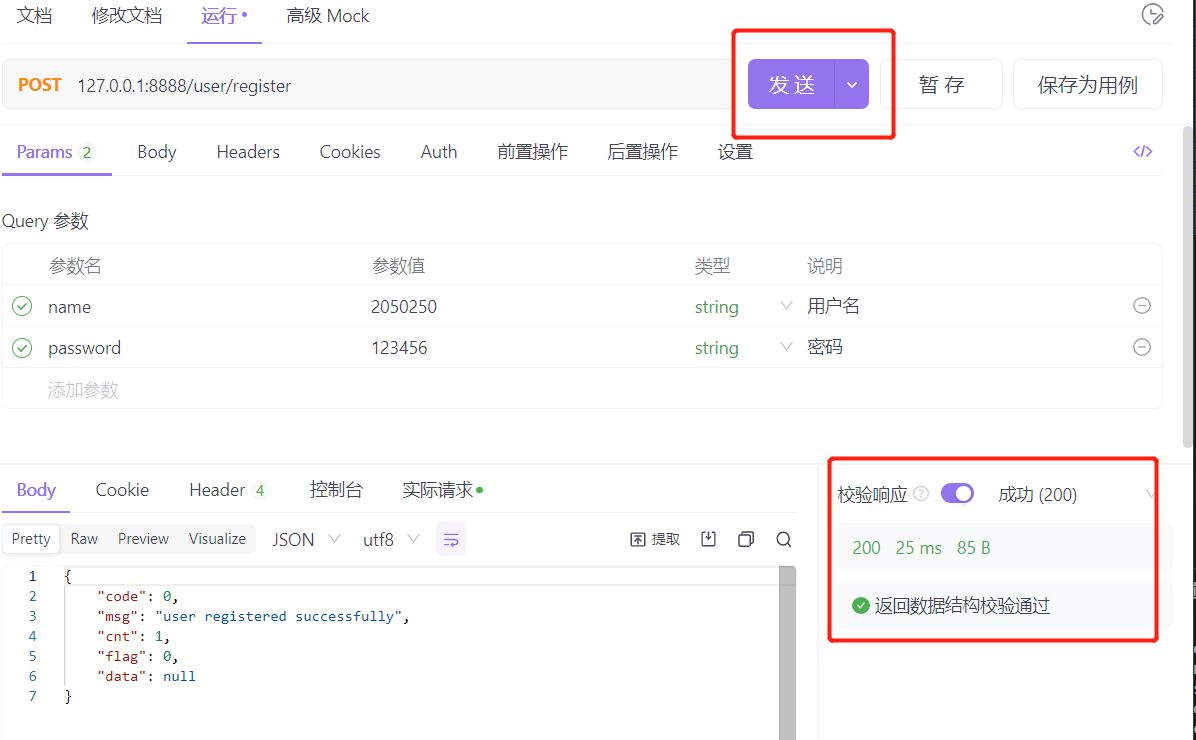
\includegraphics[width=\textwidth]{contents/figure/user_register.png}
\end{frame}


\begin{frame}
    \frametitle{单元测试}
    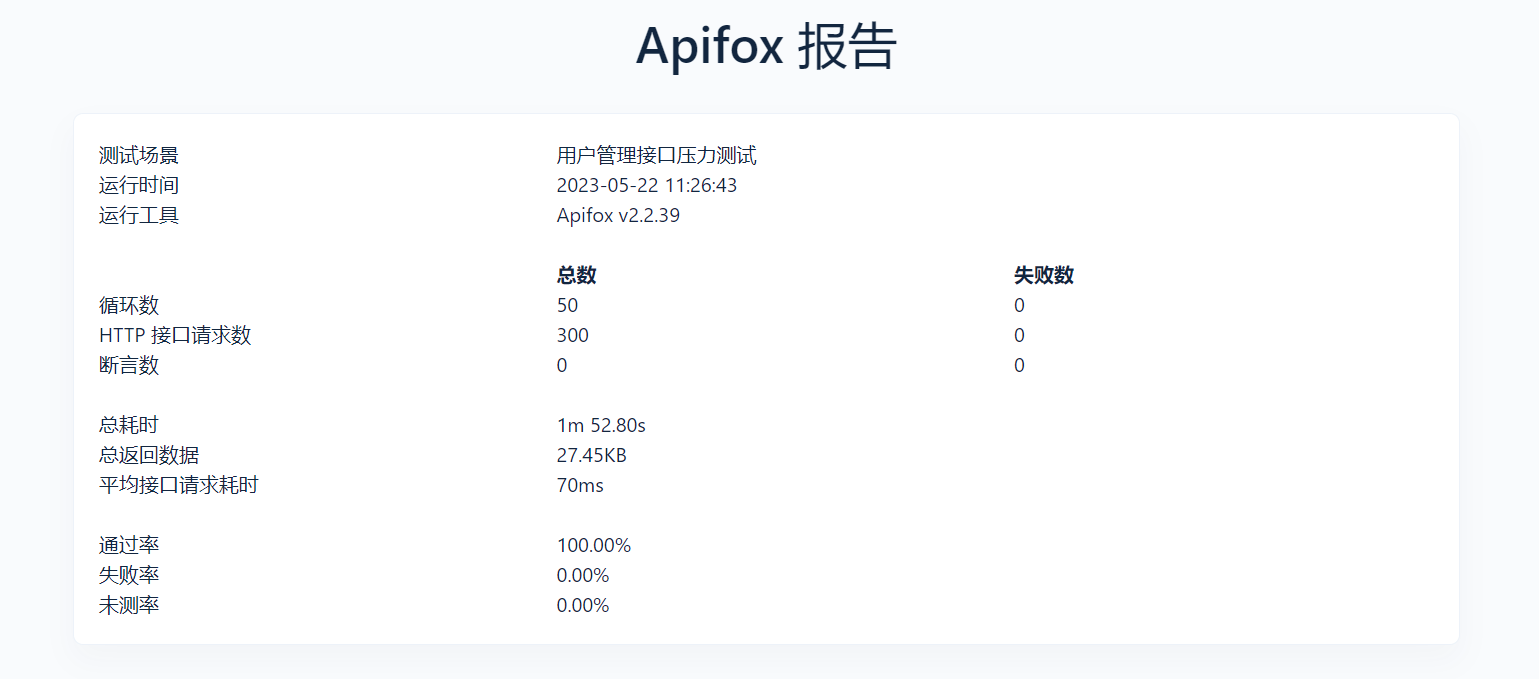
\includegraphics[width=\textwidth]{contents/figure/user_register_2.png}
\end{frame}

\begin{frame}
    \frametitle{集成测试}
    随后,在对于所有的功能接口进行单元测试正确无误后,我同样使用Apifox测试工具,对于系统进行集成测试。所谓集成测试,是在上文进行的单元测试基础上,将所有模块按照设计要求(如根据结构图)组装成为子系统或系统,并且以子系统为单位进行测试工作,从而验证每个模块在经过组装后,是否依然能够正确运行。这里,我同样以用户管理功能模块中的用户注册、登录和退出登录为例,对于我进行的集成测试工作具体方法和流程进行阐述。首先,在Apifox中设计一套模拟新用户访问系统用户管理模块的具体操作逻辑,如下所示:
\end{frame}

\begin{frame}
    \frametitle{集成测试}
    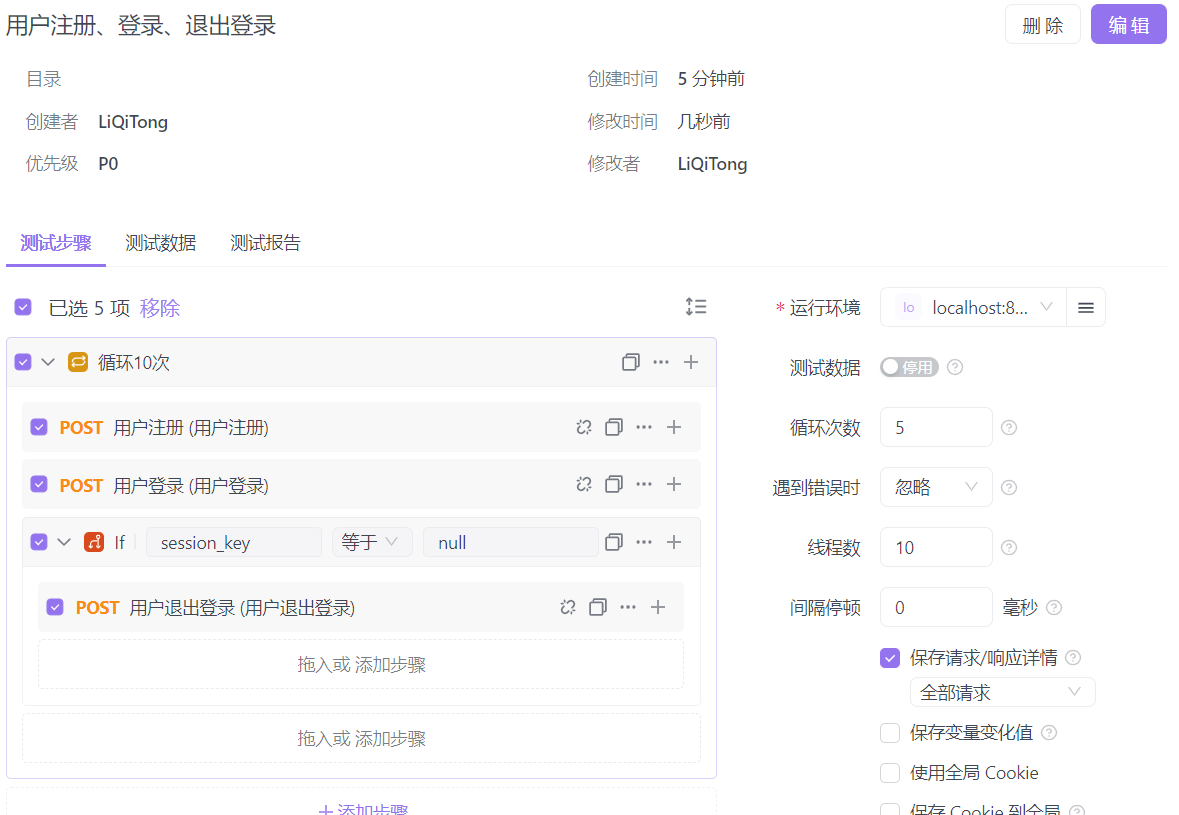
\includegraphics[width=\textwidth]{contents/figure/user_register_3.png}
\end{frame}

\begin{frame}
    \frametitle{集成测试}
    可见这里模拟了一个典型的用户访问软件系统交互逻辑,即注册新账户后登录,如果成功则储存session\_Key,访问系统其它服务,最后登出账户,在服务端的Redis缓存中相应移除用户session标识,并且更新用户stat字段为离线。该测试用例运行结果如下:
    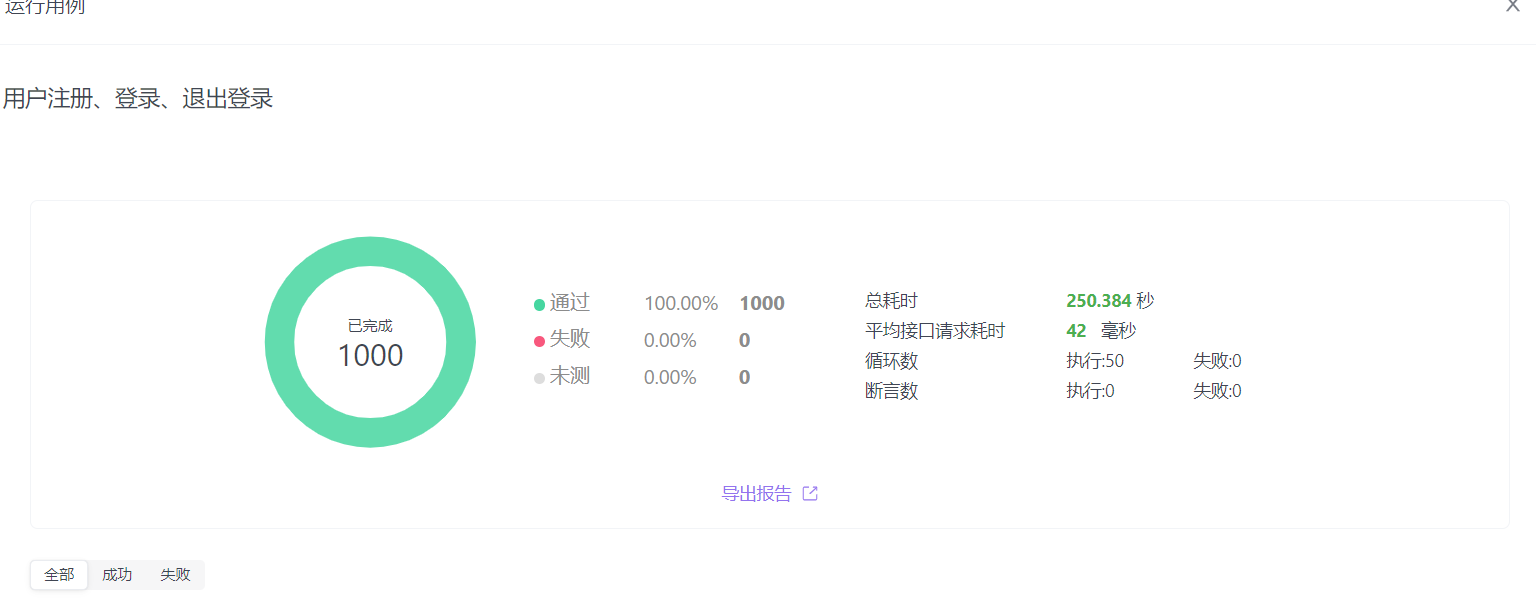
\includegraphics[width=\textwidth]{contents/figure/user_register_4.png}
\end{frame}

\begin{frame}
    \frametitle{系统测试}
    最后,在上述的两个测试阶段工作全部完成,并且测试结果验证正确无误后,我们小组的测试人员从软件系统客户端用户的角度,将实现的软件系统客户端打包发布,邀请同学和相关非开发人员的第三方用户来使用软件系统C端页面并且给出评价。同时,我们小组测试人员也对于其中C端的相关主要功能模块,从系统的层面进行了一个比较完整的用户交互逻辑测试,并且观察客户端的数据响应情况,从而能够有效地评估软件系统作为一个整体的性能表现。
\end{frame}